%!TEX TS-program = pdflatex
\documentclass{emulateapj}

\shorttitle{The Aquarius Stream Progenitor Was Not A Globular Cluster}
\shortauthors{Casey et al}

\begin{document}

\title{The Aquarius Stream Progenitor Was Not A Globular Cluster: \\ Its History Could Be Far More Interesting\altaffilmark{1}}


\author{Andrew R. Casey\altaffilmark{2,3} and distinguished collaborators}
\altaffiltext{1}{This paper includes data gathered with the 6.5 meter Magellan Telescopes located at Las Campanas Observa- tory, Chile.}
\altaffiltext{2}{Research School of Astronomy \& Astrophysics, Australian National University, Mount Stromlo Observatory, via Cotter Rd, Weston, ACT 2611, Australia; acasey@mso.anu.edu.au}
\altaffiltext{3}{Massachusetts Institute of Technology, Kavli Institute for Astrophysics and Space Research,
77 Massachusetts Avenue, Cambridge, MA 02139, USA}


\begin{abstract}
We present a detailed dynamic and chemical analysis of 5 Aquarius stream giants observed using the MIKE spectrograph on the Magellan Clay Telescope. 
\end{abstract}

\keywords{Galaxy: halo, structure --- Individual: Aquarius Stream --- Stars: FGK-giants}

\section{Introduction}

Stellar streams arise from tidal effects as satellite systems infall onto the Milky Way. The phase space information of stars within such streams are sensitive to the galactic potential. Therefore, they can collectively constrain the fraction and distribution of accreted matter in the stellar halo, the sub-halo mass function, as well as the shape and extent of dark matter in the Milky Way. Moreover, individual elemental abundances for stars within these streams help unravel the chemical evolution of the Galaxy. 
% Consider adding a final sentence about the amount of work that has gone into stellar streaams

Wide-field surveys have proved excellent sources for finding galactic substructures, including stellar streams. Dozens of streams reaching out up to 150\,kpc in the halo have been identified through photometric selections and matched-filtering techniques \citep{Belokurov;et-al_2007;Koposov_SG1}. However, as \citet{Helmi;White_1999} point out, these approaches are only successful for identifying substructures that are sufficiently distant from the solar neighbourhood. A nearby stream within $\sim{}$10\,kpc will not appear as an on-sky over-density, as the stars would be sparsely positioned across the sky. Such substructures would only be detectable with kinematic, or perhaps precise chemical information. 

% Talk about RAVE
It is therefore necessary to survey solar neighbourhood stars with spectroscopy in order to detect any nearby substructures. The RAVE (Radial Velocity Experiment) began such a survey in 2003 and has observed spectra from over 500,000 stars across 17,000 deg$^{2}$. As the name suggests, the primary goal of RAVE was to obtain radial velocities for the solar neighbourhood and beyond. In an attempt to remain kinematically unbiased, RAVE candidates were selected based only on their apparent magnitude. With the exception of bulge stars where some photometric cuts were employed, all stars between 9 $<$ I $<$ 13 were observed. Almost all of these candidates have published radial velocity measurements \citep{steinmetz;et-al_2006}, and for a subset of stars with sufficient S/N, estimates of stellar parameters have been derived using a $\chi^2$ minimization technique \citep{zwitter;et-al_2008, siebert;et-al_2011}. 

% Identification of the aquarius stream
Using these data, \citet{williams;et-al_2011} identified a co-moving group of nearby ($0.5 \lesssim d \lesssim 10$\,kpc) stars in the vicinity of the Aquarius constellation $(l, b) = (60\,^\circ, -55\,^\circ)$. The artefact is most apparent when examining kinematics against galactic latitude for stars within $-70\,^\circ < b < -50\,^\circ$. \citet{williams;et-al_2011} employed a selection criteria of $-250 < V_{HEL} < -150$\,km s$^{-1}$, $30\,^\circ < l < 75\,^\circ, J > 10.3$ to maximize the contrast between the stream and halo background, identifying 15 stream candidates in the process. The average heliocentric radial velocity of these members was found to be $V_{HEL} = -199$\,km s$^{-1}$, with a dispersion of 27\,km s$^{-1}$. The radial velocities outputted by the RAVE survey are described to be $\sim2$\,km s$^{-1}$, so the wide kinematic distribution appears to be real.

%When compared to other streams identified in the halo, this is an unusually wide kinematic dispersion. Streams are generally considered to be kinematically cold, with dispersions of $\sigma_v < 8$\,km s$^{-1}$. 

% QUANTIFYING THE STREAM DETECTION
Upon examining the galactic longitude and radial velocities of Aquarius stars, the stream appears quite distinct from the halo. In order to quantify the statistical likelihood that the Aquarius stream is a true substructure, \citet{WIlliams;et-al_2011} compared the number of observed RAVE stars within $-70\,^\circ < b < -50\,^\circ$ against the Galaxia \citep{Sharma;et-al_2009} and Besan\c{c}on \citep{Robin;et-al_2003} galaxy models. Predicted particles and observed stars between $-70\,^\circ < b < -50\,^\circ$ were binned in $\Delta{l} \times \Delta{V_{hel}}$ using varying grid cell sizes between $25-70\,^\circ$ and 20-100\,km s$^{-1}$ respectively. The significance of the stream is calculated for each cell. \citet{williams;et-al_2011} found the stream to be statistically significant ($>$4-$\sigma$) in 96\% of the grid cell sizes employed for the Besan\c{c}on model. By sampling the Galaxia model multiple times with varying extinction models, a similar result was found: between $75\pm15$\,\% to $80\pm18$\,\% of grid cells showed the Aquarius stream to significant at the 4-$\sigma$ level. Given the high-latitude of the stream and proximity of the stream, it is not surprising that dust had a negligible effect on the overall significance. \citet{williams;et-al_2011} concluded that the over-density in $l, V_{hel}$ is a true substructure, and neither the choice of galaxy model, cell size, nor the extinction model made any real difference to the stream detection significance.

% STREAM IS LOCALIZED
% the stream appears to be quite localized in space.
% nearby streams could be strewn out over several degrees. the Orphan stream wraps over 60 degrees in the sky, and the Sgr stream wraps several steradians 


% DISTANCE AND DYNAMICS
% heliocentric + galactic velocities suggest the aquarius stream stars are in the halo, and not associated with the disk.
% distances

Given the extent of stellar debris the Sagittarius dwarf has littered throughout the Milky Way, it is reasonable to suspect the Aquarius stream might originate from the Sagittarius dwarf. Indeed, the Aquarius stream stars do not lie far from the orbital plane of Sagittarius and the metallicities reported by \citet{williams;et-al_2011} are not dissimilar from the Sagittarius stream. However, \citet{williams;et-al_2011} found the Aquarius $XYZ$ positions and kinematics (specifically $V_{Z}$ and $V_\phi$) are quite distinct from Sagittarius. Based on the phase space information available, \citet{williams;et-al_2011} concluded that the newly discovered stream could not be positively associated with the Monoceros stream, Hercules-Aquila cloud, or either the Canis Major or Virgo over-densities.

The Aquarius stream has a metallicity of $\mbox{[Fe/H]} \sim -1.0$, slightly more metal-rich than halo stars at the same distance. The dispersion in the stream's metallicity has yet to be fully characterised. \citet{williams;et-al_2011} found the stream to have an average of $\mbox{[M/H]} = -1.0 \pm 0.4$, compared to $\mbox{[M/H]} = -1.1 \pm 0.6$ for background stars after the same selection cuts had been employed. Of the 12 Aquarius stars in the \citet{williams;et-al_2011} discovery sample with stellar parameters, the metallicity range is wide: between --2.02 and --0.33 dex. Spectroscopic observations of higher resolution and S/N are necessary to accurately determine the metallicity distribution function. To this end, \citet{wylie-de-boer;et-al_2012} obtained high-resolution ($R = 25,000$) spectra with modest S/N ($\sim$30 pixel$^{-1}$) for six Aquarius stream giants. Their data indicated a much narrower metallicity distribution: $\mbox{[Fe/H]} = -1.09 \pm 0.10$\,dex extending between $\mbox{[Fe/H]} = -1.25$ to $-0.98$\,dex; the level of negligible intrinsic chemical scatter which is typically observed in globular clusters. The largest [Fe/H] discrepancy between the two studies was $\Delta\mbox{[Fe/H]} = -0.66$\,dex for the most metal-rich star in the \citet{williams;et-al_2011} sample. The most metal-poor star in the \citet{williams;et-al_2011} study was not observed by \citet{wylie-de-boer;et-al_2012}.


%The chemical coherence in the \citet{wylie-de-boer;et-al_2012} study is most intriguing. 

In addition to ascertaining stellar parameters, \citet{wylie-de-boer;et-al_2012} measured light element abundances for the Aquarius stream stars -- the only study to do so until now. Primarily they focussed on Na, O, Ni, Mg, and Al abundances. Chemical patterns in these light elements arise as natural consequences of nucleosynthetic processes in massive stars. Most notably, an anti-correlation in sodium and oxygen abundance has been identified in all well-studied globular clusters to date. Originally this was thought to arise from internal mixing along the giant branch. However, dwarf stars were found to exhibit strong Na-enhancement and O-depletions, contrary to what would be expected if the Na-O anti-correlation was purely a result of internal mixing. It is well known now that photospheric abundance variations resulting from internal mixing are limited to C, N and Li. The Na-O pattern provides the best evidence that stars have formed in a globular cluster environment and that their chemical enrichment history has been dominated by Sn II events. From high-resolution spectroscopy of five stars in Aquarius, four of which had Na, O measurements, \citet{wylie-de-boer;et-al_2012} found two stars with super-solar sodium; slightly higher [Na/Fe] ratios for halo stars of the same metallicity. No strong oxygen depletion was evident in their stars.

There are other abundances patterns that allow us to infer the chemical evolution of a given cluster. \citet{Nissen;Schuster_1997} first noted that only the distant solar neighbourhood stars were enriched in [Ni/Fe] and [Na/Fe]. \citet{fulbright;et-al_2000} came to a similar conclusion: only somewhat distant ($R_\odot > 20$\,kpc) stars are likely to be sodium deficient. If the stellar halo has been built up from the accretion of smaller dwarf satellites, \citet{Nissen;Schuster_1997} proposed that this chemical trend may be indicative of the halo merger history. Although there are some caveats to this chemical pattern (see \S\ref{sec:ni-na-relation}), at the very least the Na-Ni correlation may provide an indication whether stars became chemically enriched in dSph-like environments. \citet{wylie-de-boer;et-al_2012} found all their Aquarius stars to be enriched in both sodium and nickel; contrary to what would be expected if the stars originated from a disrupted dSph satellite. 

Combined with the low level of chemical scatter present in their sample, these chemical indicators led \citet{wylie-de-boer;et-al_2012} to conclude that the Aquarius stream must be the result of a tidally disrupted globular cluster. \citet{williams;et-al_2011} had previously precluded this possibility after modelling an Aquarius-like progenitor infalling onto the Milky Way and comparing the predicted $l, b, V_{hel}$ with known, nearby globular clusters of similar metallicities. However, no known globular cluster could match their simulation. 

We seek to investigate the nature of the Aquarius stream, in particular the recent globular cluster origin claim made by \citet{wylie-de-boer;et-al_2012}. We present a detailed analysis for five confirmed Aquarius stream members from high-resolution, high S/N observations taken using the Magellan Inamori Kyocera Echelle spectrograph \citep{Bernstein;et-al_2003} on the Magellan Clay telescope. Our analysis includes determining the galactic dynamics and orbital paths for the Aquarius stream, and measuring precise chemical abundances. Details of the observations and data reduction are outlined in the following section. The data analysis is chronicalled in \S\ref{sec:analysis} and a detailed discussion of these results resides in \S\ref{sec:discussion}. In \S\ref{sec:conclusion} we present our conclusions and critical interpretations.

\clearpage
\section{Observations \& Data Reduction}


The most comprehensive sample of Aquarius stream stars is presented in the discovery paper of \citet{williams;et-al_2011}. Our sample includes five stars: four common to the \citet{wylie-de-boer;et-al_2012} study, and an additional star from the original \citet{williams;et-al_2011} sample. The additional star, J2306265-085103, had insufficient S/N in the RAVE sample for stellar parameters to be accurately determined. Program stars were observed in July 2011 in good seeing at high airmass (Table \ref{tab:observations}), and X standard stars were observed as part of a separate program in March 2011. All observations were taken using the 1.0'' slit, providing a spectral resolution of $R = 28,000$. The exposure times for our program stars varied per star from X-Y seconds to ensure a Signal-to-Noise ratio (S/N) in excess of 100 per pixel element at 600 nm.



Calibration frames were taken at the start of each night, including twenty flat-field frames (10 quartz, 10 milky) and 10 Th-Ar arc lamp exposures for wavelength calibration. The data were reduced using the CarPy pipeline\footnote{carpy website url}. One of our standard stars, HD 41667, was also reduced using standard extraction and calibration methods in \textsc{IRAF}. The resultant spectra from both reduction workflows were compared for residual fringing, S/N, and wavelength calibration. No noteworthy differences were present, and the CarPy pipeline was utilized for the remainder of our reductions. Each reduced echelle order was carefully normalised using a third order spline. Normalised orders  for a given star were stitched together to provide a single one-dimensional spectrum from 3800-9400\,\AA{}. 
 
The white dwarf HR 6141 was observed on X with a S/N of 400 pixel$^{-1}$ to account for telluric absorption. The S/N for HR 6141 exceeds the S/N in any of our program stars. Although the atmospheric conditions are certain to change throughout the night and between observing runs, we are primarily using this spectra to identify lines that are affected by telluric absorption. Critical transitions necessary for abundance analyses that are affected by the earth's atmosphere are later corrected for telluric absorption (see \S\ref{sec:telluric-absorption}), but great attention is paid to telluric band-heads at X and X such that we are not over- or under-correcting the atmospheric absorption.

\begin{deluxetable*}{lcccccccccc}
\tablecolumns{1}
\tabletypesize{\scriptsize}
\tablecaption{Observations\label{tab:observations}}
\tablehead{
	\colhead{Designation} &
	\colhead{$\alpha$} &
	\colhead{$\delta$} &
	\colhead{Observed} &
	\colhead{Airmass} &
	\colhead{Seeing} &
	\colhead{$t_{exp}$} &
	\colhead{S/N\tablenotemark{a}} &
	\colhead{$V_{rad}$} &
	\colhead{$V_{hel}$} &
	\colhead{$V_{err}$} \\
 & (J2000) & (J2000) & Date & & (") & (secs) & (px$^{-1}$) & (km s$^{-1}$) & (km s$^{-1}$) & (km s$^{-1}$)
}
\startdata

C2225316-14437	& 22:25:31.7 & $-$14:54:39.6	& 2011-07-30	& 1.033 & \dots & \dots & \dots & $-$169.0	& \dots & 0.7 \\
C2306265-085103	& 23:06:26.6 & $-$08:51:04.8	& 2011-07-30	& 1.096 & \dots & \dots & \dots & $-$239.3	& \dots & 0.6 \\
HD41667			& 06:05:03.7 & $-$32:59:36.8	& 2011-03-13	& 1.005	& \dots & \dots & \dots & 314.4	& \dots & 0.8 \\
HD142948		& 16:00:01.6 & $-$53:51:04.1	& 2011-03-14	& 1.107	& \dots & \dots & \dots & 6.8		& \dots & 0.4 \\
J221821-183424	& 22:18:21.2	& $-$18:34:28.3	& 2011-07-30	& 1.026	& \dots & \dots & \dots & $-$170.5	& \dots & 0.5 \\
J223504-152834	& 22:35:04.5	& $-$15:28:34.9	& 2011-07-30	& 1.047	& \dots & \dots & \dots & $-$180.9	& \dots & 0.7 \\
J223811-104126	& 22:38:11.6	& $-$10:41:29.4	& 2011-07-30	& 1.218	& \dots & \dots & \dots & $-$248.4	& \dots & 0.7 

\enddata
\tablenotetext{a}{S/N measured at 6000 \AA{} for each target.}
\end{deluxetable*}


\section{Analysis}
\label{sec:analysis}

\subsection{Radial Velocities}
\label{sec:radial-velocities}
The radial velocity for each star was determined in a two-step method. An initial estimate of the radial velocity was ascertained by cross-correlation with the synthetic spectrum of a giant with $T_{eff} = 4500$\,K, $\log{g} = 1.5$, and [M/H] $= -1.0$ across the wavelength range $8450 - 8700$ \AA{}. The observed spectrum was shifted to the pseudo-rest frame using this initial velocity. Velocities found from cross-correlation are typically within 1\,km\,s$^{-1}$ of our final published value.

With our spectrum at near-rest, we measured the equivalent widths of $\sim$200 lines by fitting Gaussian functions to the absorption profiles. Fitted Gaussian profiles provides us with a measured equivalent width, the full-width half-maximum of the profile, and the central wavelength. Thus, the residual radial velocity can be found from the ratio of the central and rest line wavelengths. The final radial velocity for the star is provided by the mean of these $\sim$200 line velocity measurements. Figure \ref{fig:line-velocities} shows the line velocities for HD41667 after being placed at pseudo-rest using our cross-correlation velocity of 314.4\,km s$^{-1}$. As expected, the mean residual offset is small ($-0.75$\,km s$^{-1}$), and our standard deviation is 0.79\,km s$^{-1}$ from 164 line measurements. This provides us with a final measured radial velocity of $313.7 \pm 0.1$\,km s$^{-1}$. This process was performed for all observations. The radial velocities published in Table \ref{tab:observations} are the final values from this two-step method. Heliocentric velocities agree excellently (within X\,km s$^{-1}$) with previously reported literature values \citep{williams;et-al_2011,wylie-de-boer;et-al_2012}, demonstrating the accuracy of the radial velocities published by the RAVE survey.

\begin{figure}[h]
	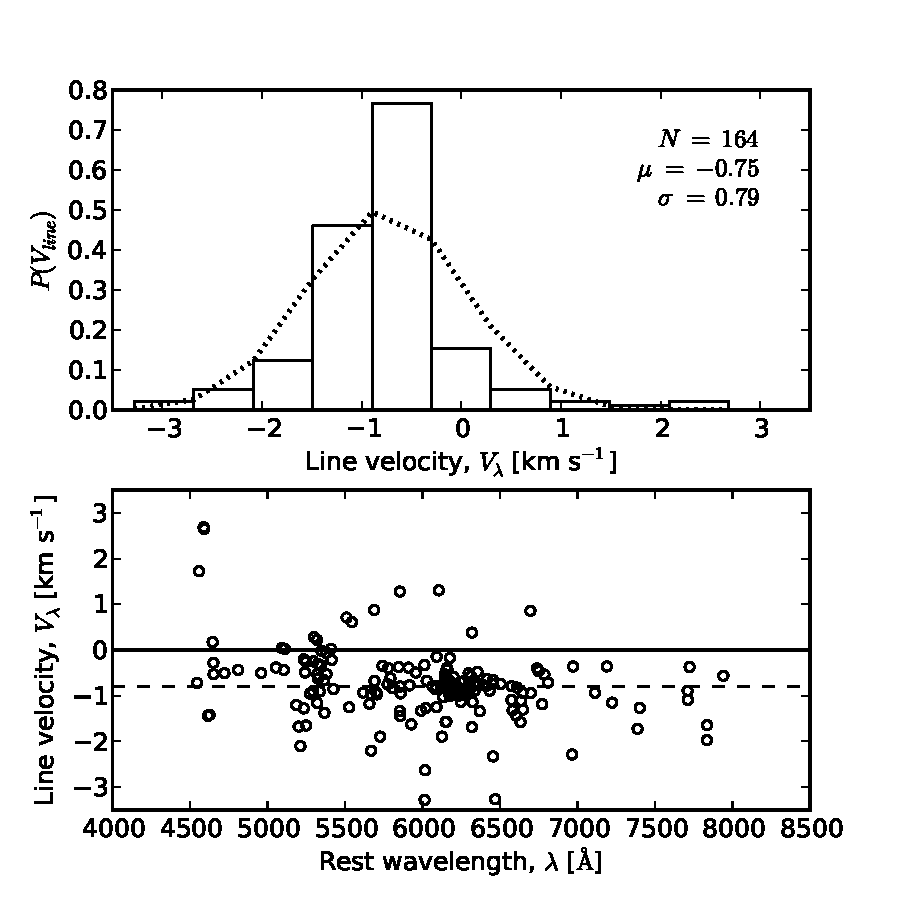
\includegraphics[width=\columnwidth]{./figures/line-velocity.pdf}
	\caption{Residual velocities for each absorption line with a well-fitted Gaussian profile after correcting for  doppler shift with our initial cross-correlation measurement. The mean residual velocity $-0.75$\,km\,s$^{-1}$ is within the 1-$\sigma$ cross-correlation uncertainty of $\pm0.9$\,km\,s$^{-1}$.}
	\label{fig:line-velocities}
\end{figure}


\subsection{Line Measurements}
\label{sec:line-measurements}

For the measurement of atomic absorption lines, we employed the line list of \citet{yong;et-al_2005} with additional transitions of Cr, Sc, Zn, and Sr from \citet{frebel;et-al_2010}. We supplemented the list with hyperfine-structure data for Sc and Mn from the Kurucz compilation \citet{Kurucz;1998}. Molecular line data for CH was taken from \citet{Plez;et-al_2008,Plez;et-al_2009}. For lines with hyperfine structure, blended transitions or molecular features, we determined the transition abundance using a spectral synthesis approach where the abundance of a given species is found by by matching a synthetic spectrum to the observed spectrum. Equivalent widths were measured to determine the abundances of all other transitions.

The equivalent widths for all absorption lines were measured automatically using software written for this study. Given the rest wavelength and an initial guess of the full-width half-maxium (FWHM), a Gaussian function is iteratively fitted to the absorption profile. At the same time, the local continuum is found within 20\,\AA{} either side of the rest wavelength using a second-order polynomial. Measuring the local continuum ensures any errors in our initial normalisation or order-stitching do not propagate through to our equivalent width measurements. Any group of pixels that deviate significantly ($>$2-$\sigma$) from the local continuum are either persistent cosmic ray hits, or trough points of a neighbouring absorption profile. We attempt to fit a Gaussian profile to each group of deviating pixels, using the current best estimate for the local continuum. If a Gaussian profile is successfully fitted to the deviating group and its surrounding pixels, then all points belonging to that profile are excluded from the continuum determination. When fitting Gaussian profiles, the $\chi^2$ difference between the observation and the profile is minimized. In order to account for crowded absorption regions where the $\chi^2$ value might be influenced by a nearby profile, our $\chi^2$ function is weighted based on the distance to the rest wavelength by the function

\begin{equation}
W_{\lambda_{i}} = 1 + \exp{\left(\frac{-(\lambda_{i} - \lambda_{r})^2}{4\sigma^2}\right)}
\label{eq:chi-weight}
\end{equation}

\noindent where $\lambda_{r}$ (rest wavelength) and $\sigma$ are free parameters during the iterative fitting process. As a consequence of Eq. \ref{eq:chi-weight}, pixels near the rest wavelength are weighted higher than those on the wings, forcing the fit to disregard blended or crowded regions. Although this approach relies on a reasonably accurate radial velocity correction ($<$4\,km s$^{-1}$; which is easily achieved), it greatly improves the accuracy of the equivalent width measurements.

We note that the results of our iterative fitting approach are \textit{completely insensitive} to the initial FWHM guess. Increasing the initial FWHM estimate from 0.1\,\AA{} to 1 or 2\,\AA{} -- unphysically large values for high-resolution spectra -- does not alter \textit{any} of our final equivalent width (or FWHM) measurements. Only a small increase in computational cost is observed. Although we are extremely confident in our automatic equivalent width measurements, every absorption profile was examined by eye for quality, and spurious measurements were excluded.

We list the atomic data and measured equivalent widths for atomic lines used during this analysis in Table \ref{tab:equivalent-widths}. Saturated lines were excluded by removing measurements with reduced equivalent widths, $\log_{10}{(EW/\lambda)} > -4.5$\, dex. A minimum detectable equivalent width was calculated as a function of wavelength based on the S/N, and only lines that exceeded a $3\sigma$ detection significance were included. We have verified our equivalent width measurement techniques by comparing our measurements for 164 lines in HD140283 with the study of \citet{norris;et-al_1996}. Excellent agreement is found between the two studies, which is illustrated in Figure \ref{fig:ew-compare}. The mean difference between this study and that of \cite{norris;et-al_1996} is a negligible $0.64 \pm 2.78$\,m\AA{}, and no systematic trend is present. 

% need to mention that we only used the "Good" Norris measurements

% equivalent widths plot with Norris for HD 122563
\begin{figure}[h]
	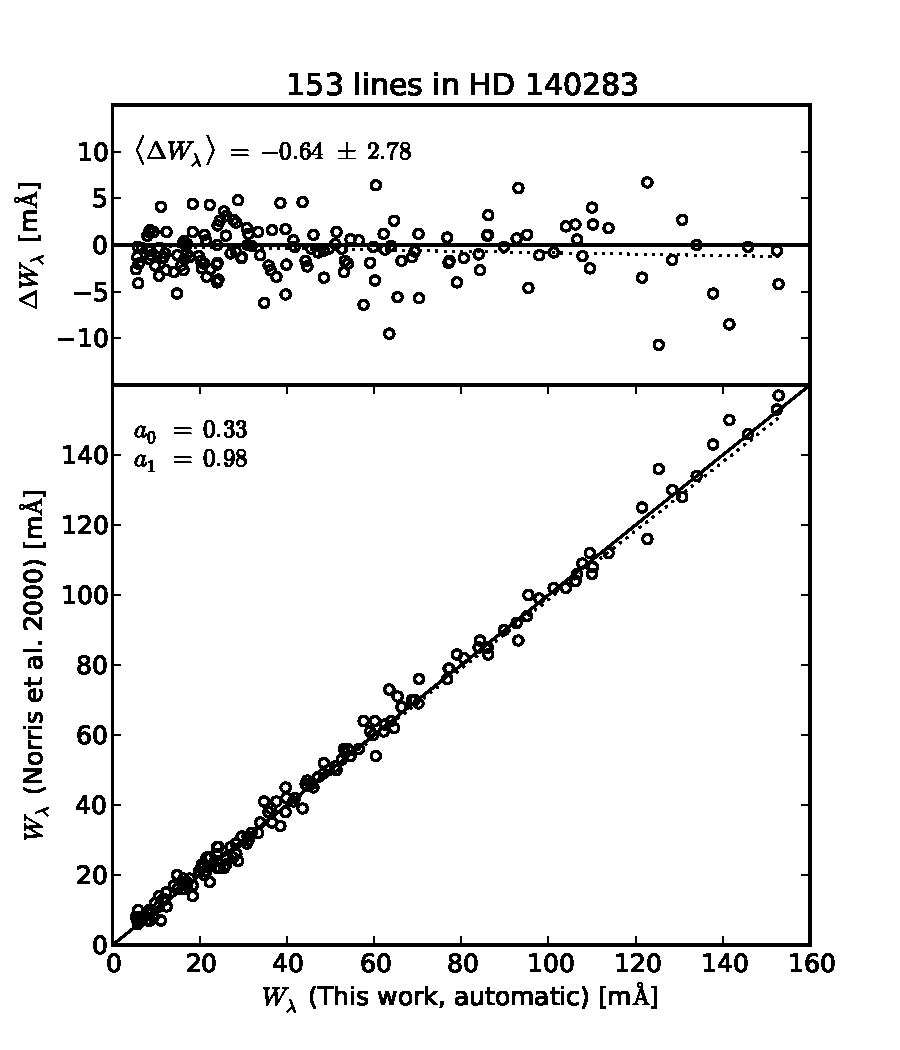
\includegraphics[width=\columnwidth]{./figures/smh-norris.pdf}
	\caption{A comparison showing equivalent widths measured for HD140283 using our automatic routine (see \S\ref{sec:line-measurements}), and those found with careful hand measurements by \citet{norris;et-al_1996}. No systematic trend is present, and the mean difference between these studies is $\langle\Delta{}W_\lambda\rangle = -0.64 \pm 2.78$ m\AA{}.}
	\label{fig:ew-compare}
\end{figure}


% equivalent widths table

\subsection{Model Atmospheres}
The ATLAS9 plane-parallel stellar atmospheres of \citet{Castelli;Kurucz_2003} have been used to deduce stellar parameters and abundances for all of our stars. These one-dimensional models ignore any centre-to-limb spatial variations, assume hydrostatic equilibrium and no convective overshoot from the photosphere. The stellar parameter spacing for these grid models is 250\,K, 0.5\,dex in surface gravity, 0.5\,dex in [M/H] and 0.1\,dex in [$\alpha$/Fe]. We interpolated the atmospheric pressures, densities, temperatures, and opacities between stellar atmospheres using the Quickhull algorithm \citep{Barber;et-al_1996}. Quickhull is reliant on Delaunay tessellation, which suffers from extremely skewed cells when the grid points vary in size by orders of magnitude -- as $T_{\mbox{eff}}$ values do compared to $\log{g}$ or [X/H]. If unaccounted for, performing interpolation using these asymmetric cells can manifest as significant errors in atmospheric properties across all photospheric depths. We scaled each stellar parameter between zero and unity prior to interpolation in order to minimise these errors. During this step, $\log{g}$, [M/H] and [$\alpha$/Fe] points were scaled such that we simultaneously interpolate linearly in $T_{eff}$ and logarithmically in all other parameters.

\subsection{Stellar Parameters}
The most recent version of the spectral synthesis code MOOG \citep{Sneden;et-al_1973} has been used to derive individual line abundances and stellar parameters. This version of MOOG employs Rayleigh scattering \citep{Sobeck;et-al_2011} instead of treating scattering as true absorption, which is particularly important for transitions blue-ward of 450\,nm. This is noteworthy, but is less relevant for this analysis as most of our line measurements are red-ward of 450\,nm. Absorption lines are assumed to form under the assumption of local thermal equilibrium. 

\subsubsection{Effective Temperature}

The effective temperature for each star was found by demanding a zero-trend in excitation potential and abundance for each measured Fe\,I line. In the same way, the microturbulence was found by demanding a zero trend in reduced equivalent width against abundance. Linear relationships with slopes of $|0.001|$ dex were considered to be converged. 

\subsubsection{Photometric Effective Temperatures}
\label{sec:photometric-temperatures}

The effective temperatures published for all of our stars in Table \ref{sec:stellar-parameters} have been derived spectroscopically (see \S\ref{sec:effective-teffs}). As a consistency check for our spectroscopic temperatures, we have also estimated effective temperatures using infrared photometry from the 2MASS catalog. The $J-K$ colour has been employed for these calculations because it has the least dependence on metallicity. 

The Aquarius stream is relatively close and at high-latitude, so significant extinction by dust is not expected. The dust maps of \citet{Schlegel;et-al_1998} estimate that the extinction for our stars varies between E(B-V) = 0.03 to 0.07 mags. However, these maps are not perfect. As an alternative to using the \citet{Schlegel;et-al_1998} dust maps, the level of extinction towards a star can be found by the strength of their interstellar Na D or K \textsc{I} lines \citep{Munari;Zwitter_2006}. The interstellar lines must be sufficiently separated from the stellar lines in order for the extinction to be measurable. Unfortunately this was the case in only one of our stars, J223811. We measure the equivalent width of the Na D \textsc{I} line in J223811 to be 302.4\,m{\AA}, which corresponds to an $\mbox{E(B-V)} = 0.12^{+0.01}_{-0.02}$ according to the \citet{Munari;Zwitter_2006} relationship. This is a significantly higher value than what the \citet{Schlegel;et-al_1998} dust map value of $\mbox{E(B-V)} = 0.07$ for J223811. Both extinction values have been used to calculate photometric temperatures. 

Although all of our targets are giant stars, two different $T_{eff}$-colour relationships have been employed: the \citet{Alonso;et-al_1999} calibration for giants, and the \citet{Casagrande;et-al_2010} calibration for dwarfs and sub-giants. All photometrically-derived temperatures are listed in \ref{tab:photometric-temperatures}. The \citet{Alonso;et-al_1999} $J-K$ scale is insensitive to metallicity effects, and is in good agreement with our spectroscopic temperatures. For the \citet{Casagrande;et-al_2010} $J-K$ relationship, which has a slight metallicity dependency, we have utilized the spectroscopically-derived [Fe/H] values shown in Table \ref{tab:stellar-parameters}.

The effective temperatures that we have found from spectroscopy agree fairly well with the photometric temperature estimates. For three of our stars, the temperatures we find are in between the two color-temperature relationships. There are two noteworthy deviations though: J223504-152834 and J223811-104126. For J223504-152834 we find the star to have an effective temperature of 4620\,K, 40\,K hotter than the \citet{Casagrande;et-al_2010} dwarf/sub-giant relationship, and ${\sim}$500\,K hotter than the \citet{Alonso;et-al_1999} temperature. Our temperature of 4620\,K is in good agreement with previous spectroscopic determinations (4795\,K; \citet{williams;et-al_2011}, 4597\,K; \citet{wylie-de-boer;et-al_2012}). The fact that the \citet{Alonso;et-al_1999} photometric temperature relationship for giants predicts a temperature that is ${\sim}$500\,K cooler than the spectroscopically-derived values may be attributed to an underestimated amount of dust towards J223504-152834. A higher than expected level of extinction along the line-of-sight would produce cooler temperatures than the true effective temperature. 

The F-giant J223811-104126 has two extinction values available: the \citet{Schlegel;et-al_1998} value of $E(B-V) = 0.07$ and the 0.12 value that we have determined from the interstellar Na D1 line. Given the inherent difficulties in producing dust maps, and the known problems associated with them, we believe the $E(B-V) = 0.12$ determination to be more accurate. However, using the \citet{Schlegel;et-al_1998} extinction with the \citet{Alonso;et-al_1999} color-temperature relationship yields excellent agreement (within 6\,K) with our spectroscopic temperatures. Employing our more accurate reddening determination yields 5215\,K, within the uncertainties of the relationship. The \citet{Casagrande;et-al_2010} scale is ${\sim}$250\,K hotter in both cases.

Thus, with the exception of J223504-152834, the \citet{Alonso;et-al_1999} giant relationship agrees well ($\pm$100\,K) with our spectroscopically derived values. The \citet{Casagrande;et-al_2010} relationship is also in relatively good agreement with our spectroscopic temperatures, although we note that this relation was derived primarily for dwarfs/sub-giants. The discrepancy in J223504-152834 could very well be due to under-estimated reddenning along the line-of-sight. An extinction of $E(B-V) = 0.10$ would be required for the \citet{Alonso;et-al_1999} relation to yield a temperature of ${\sim}$4500\,K, within the uncertainties of our effective temperature derived from spectroscopy. Such a discrepancy in extinction is large, but not unheard of (e.g., the case of J223811-104126 or see \citet{Nataf;et-al}). Although we suspect J223504-152834 to have a higher reddening than $E(B-V) = 0.04$, we have adopted the \citet{Schelegel;et-al_1998} value for this analysis.

\begin{deluxetable}{lccccc}
\tablecolumns{1}
\tabletypesize{\scriptsize}
\tablecaption{Reddening \& Photometric Temperatures}
\tablehead{
& & & \multicolumn{2}{c}{$T_{phot}$} \\
\cline{4-5} \\
	\colhead{Designation} &
	\colhead{E($B-V$)} &
	\colhead{$(J-K)_0$} &
	\colhead{Alonso} &
	\colhead{Casagrande} \\
	& (mag) & & (K) & (K)
}
\startdata 
C222531-144370 	& 0.03\phn	& 	0.75 & 4247	&	4391 \\	
C230626-085103	& 0.05\phn	&	0.82 & 4091	&	4200 \\	
J221821-183424 	& 0.03\phn	&	0.64 & 4546	&	4747 \\	
J223504-152834 	& 0.04\phn	&	0.69 & 4110	& 	4579 \\	
J223811-104126 	& 0.07\phn	&	0.48 & 5104	&	5367 \\	
				& 0.12\footnote{Extinction derived from interstellar Na D1 line (see \ref{sec:photometric-temperatures})} 			&	0.45 & 5215	&	5484	
\enddata
\end{deluxetable}

\subsubsection{Surface Gravity}

Surface gravity was found by forcing the mean Fe\,I and Fe\,II abundances to be equal, whilst maintaining zero trends with the excitation potential, reduced equivalent width and abundance. After these parameters had converged, the model metallicity was exactly matched to that of our line abundances. Line abundances that were unusually deviant ($3\sigma$) from the mean were removed. The largest number of outlier measurements removed for any observation was N for X.

\subsubsection{Metallicity, $\mbox{[M/H]}$}
Determining the stellar parameters for a given star is an iterative process. Once the effective temperature, microturbulence and surface gravity were deduced, the model atmosphere abundance was matched to our solar-scaled Fe \textsc{I} abundance. The degeneracy between parameters required a refinement of the stellar parameters until the line abundances were consistent with the model atmosphere.

% process is iterative
% our final Fe abundance matched the model atmosphere abundance


% spectral plots for five stars

\begin{deluxetable*}{lcccccccccccccc}
\tablecolumns{2}
\tabletypesize{\scriptsize}
\tablecaption{Stellar Parameters}
\tablehead{
	\colhead{Designation} &
	\colhead{$T_{eff}$} &
	\colhead{$\log{g}$} &
	\colhead{$v_t$} &
	\colhead{[Fe/H]} & 
	\colhead{$T_{eff}$} &
	\colhead{$\log{g}$} &
	\colhead{$v_t$} &
	\colhead{[Fe/H]} &
	\colhead{Source} \\
	& (K) & (dex) & (km\,s$^{-1}$) & (dex) & (K) & (dex) & (km s$^{-1}$) & (dex) 
}
\startdata
\multicolumn{10}{c}{Standard Stars} \\
\cline{1-10} \\
HD41667			& 4630	& 1.70	& 1.66 	& --1.21
				& 4605	& 1.88	& 1.44	& --1.16
				& \citet{gratton;et-al_2000} \\
HD44007			& 4790	& 1.78	& 1.63	& --1.80
				& 4850	& 2.00 	& 2.20	& --1.71
				& \citet{fulbright_2000} \\
HD142948		& 4950	& 2.19	& 1.78	& --0.79
				& 4713 	& 2.17 	& 1.38	& --0.77
				& \citet{gratton;et-al_2000} \\
\\
\multicolumn{10}{c}{Program Stars} \\
\cline{1-10} \\
C2225316-14437	& 4350	& 1.60	& 1.80	& --1.19	
				& 4235 $\pm$ 118 & 1.45 $\pm$ 0.21 & 1.96 $\pm$ 0.11 & --1.20 $\pm$ 0.14 
				& \citet{wylie-de-boer;et-al_2012} \\
C2306265-085103	& 4180	& 1.00	& 1.80 	& --1.16
				& \dots	& \dots	& \dots	& \dots
				& \dots \\	
J221821-183424	& 4570	& 0.80	& 1.93	& --1.60
				& 4395 $\pm$ 205 & 1.45 $\pm$ 0.35 & 1.96 $\pm$ 0.18 & --1.15 $\pm$ 0.21
				& \citet{wylie-de-boer;et-al_2012} \\
J223504-152834	& 4620	& 2.15 	& 1.44	& --0.65
				& 4597 $\pm$ 158 & 2.40 $\pm$ 0.14 & 1.47 $\pm$ 0.07 & --0.98 $\pm$ 0.17
				& \citet{wylie-de-boer;et-al_2012} \\
J223811-104126	& 5100	& 3.00	& 1.21	& --1.44
				& 5646 $\pm$ 147 & 4.60 $\pm$ 0.15 & 1.09 $\pm$ 0.11 & --1.20 $\pm$ 0.20
				& \citet{wylie-de-boer;et-al_2012} 
\enddata

\end{deluxetable*}


\subsection{Abundances}
We have scaled our abundances to solar values using the chemical composition of \citet{Asplund;et-al_2009}.

\subsubsection{Carbon}

\subsubsection{Oxygen}
\label{sec:oxygen-abundances}
Oxygen is a particularly difficult element to measure. There are only a handful of lines available in an optical spectrum: the forbidden [O \textsc{I}] lines at 630 nm and 636 nm, and the O \textsc{I} triplet lines at 777 nm. The forbidden lines are very weak, and become immeasurable in either hot and/or metal-poor stars ([Fe/H] $\lesssim -1.5$ dex). When they are present, depending on the radial velocity of the star, the [O \textsc{I}] can be significantly affected by telluric absorption. Moreover, the 630 nm line is blended with a Ni \textsc{I} absorption line \citep{Allende-Prieto;et-al_2001}, and hence the region requires careful consideration. Although the O \textsc{I} triplet lines at 777 nm are stronger than the forbidden lines, they are extremely susceptible to NLTE and 3D effects \citep{Asplund;Perez_2001}, and sensitive to changes in microturbulence. \citet{Perez;et-al_2006} showed that oxygen abundances measured under the assumption of LTE in their sample are 0.08\,dex higher than abundances derived from the `true' oxygen content derived from the forbidden lines \citep{Perez;et-al_2006}. 

The [O \textsc{I}] lines were measurable in four of our candidates. Careful consideration was taken when correcting for telluric absorption, and we inspected all lines for any contamination by the earth's atmosphere. The 6300$\lambda$ line in one of our candidates, C2306265-085103, was sufficiently affected by telluric absorption such that we considered the line immeasurable. Thus, only the 6363$\lambda$ line was used to derive an oxygen abundance for C2306265-085103. In our hottest star, J223811-104126, the forbidden oxygen lines were not detected above a $3-\sigma$ significance. After synthesising the region, we deduce a conservative upper limit of $\mbox{[O/Fe]} < -0.50$ dex from the [O \textsc{I}] lines. This is consistent with the rest of our candidates, with [O/Fe] abundances varying between 0.41 to 0.57 dex.

In order to derive an oxygen measurement for J223811-104126, we were forced to use the triplet lines at 777\,nm. Each line was synthesised, and a mean abundance was calculated for each candidate. Abundances determined from the oxygen triplet lines were systematically $+0.27$\,dex higher than found from the [O \textsc{I}] lines. \citet{Perez;et-al_2006} found [O/Fe] values based on the O \textsc{I} permitted triplet lines are on average $+0.19 \pm 0.07$\,dex higher than those found from the forbidden lines, after NLTE corrections of $-$0.08\,dex had been applied.  Thus, our 0.27\,dex offset between measurements of the [O \textsc{I}] and O \textsc{I} triplet lines is exactly the same as found by \citet{Perez;et-al_2006}, which we attribute to a combination of NLTE, 3D and other systematic effects. \citet{Perez;et-al_2006} concluded the weak forbidden lines, when not too weak, probably give the most reliable estimate of [O/Fe].

From the permitted O \textsc{I} triplet, we derive an oxygen abundance of $\mbox{[O/Fe]} = 0.41 \pm 0.01$\,dex (random scatter) for J223811-104126. This measurement will be systematically higher than the `true' abundance if it were discernible from the [O \textsc{I}] lines, on the order of $\sim{}$0.27\,dex. When we apply this crude offset derived from the rest of our sample, we arrive at a corrected abundance of $[O/Fe] = 0.14 \pm 0.08$\,dex for J223811-104126. This is the most oxygen-deficient star in our sample.


\subsubsection{Sodium}

Sodium is mainly produced through through carbon burning in massive stars by the dominant $^{12}\mbox{C}(^{12}\mbox{C}, p)^{23}\mbox{Na}$ process. The final Na abundance is dependent on the neutron excess of the star, which slowly increases during carbon burning due to weak interactions \citep{Arnett;Truran_1974}. Massive stars ($>8 M_\odot$) eventually deliver their manufactured sodium to the interstellar-medium through SN II events. Because the eventual SN II explosion is devoid of any significant beta-decay processes, the neutron excess of the exploded material is representative of the pre-explosion abundance.  
  
The explosive material eventually condenses to form the next generation of stars, which will have a net increase in their neutron excess with respect to when their predecessors formed. Since the Na-production rate is correlated with the neutron excess, an overall increase in the total Na and Na-production rate between stellar generations is expected. Thus, an increase in the Na abundance between generations of massive stars is a natural consequence of nucleosynthesis. Sodium content also becomes important for production of Ni during the SN II event (see \S\ref{sec:na-ni}) because $^{23}$Na is the only stable isotope produced in significant quantities during the C- (or O-) burning stages. A small fraction of $^{22}$Na is also forged through proton capture on $^{21}$Ne in the carbon shell, an effect which is enhanced by neutrinos spallating abundant elements like $^{16}$O and $^{20}$Ne, making free protons available for capture \citep{Woosley;Weaver_1995}.

% which lines did we use for sodium and were there any problems with the Na lines? 

\subsubsection{$\alpha$-elements (Mg, Ca, Si and Ti)}
\label{sec:alpha-elements}

The $\alpha$-elements (Mg, Ca, Si and Ti) are forged through $\alpha$-particle capture in assorted burning stages of stellar evolution, including the burning of carbon, neon and silicon. Although Ti ($Z = 22$) is not formally an $\alpha$-element, its abundance generally varies with those of the other $\alpha$-elements and therefore has been included here.

% magnesium measurements
%Magnesium has been measured from unblended lines that fall within the linear regime between reduced equivalent width and abundance.
Depending on the radial velocity of the star, some magnesium lines were be affected by telluric absorption, particularly the 6318$\lambda$ and 6965.4$\lambda$ lines. Atmospheric absorption was most notable for C2225316-14437, where three of the four Mg transitions in our line list suffered some degree of telluric absorption, requiring an attentive correction. Every amended absorption profile was carefully examined, and lines with suspicious profiles were excluded from the final magnesium abundance.

% calcium measurements + silicon measurements
Of all the $\alpha$-elements, calcium has the smallest measurement scatter in our stars. Four line measurements were used for each star, with a measurement uncertainty of 0.01\,dex. As shown in Figure \ref{fig:alpha-elements}, all Aquarius stars show super-solar Ca abundances, ranging between 0.23 to 0.43 dex, consistent with both [Mg/Fe] and [Si/Fe] measurements. However, C2225316-14437 has an unusually high silicon abundance ($\mbox{[Si/Fe]} = 0.72$), well outside the uncertainties of the rest of our sample. C2225316-14437 does not demonstrate unusually high abundances of any other $\alpha$-element, and the silicon lines are not affected by telluric absorption. Moreover, the Si lines are in relatively good agreement with one another. If we exclude the most prominent outlier, then the mean abundance drops only slightly to $\mbox{[Si/Fe]} = 0.70 \pm 0.04$\,dex. The lowest silicon line abundance for C2225316-14437 is $\mbox{[Si/Fe]} = 0.57$\,dex, still significantly higher than the final measurements for any other star.

% titanium measurements

\subsubsection{Iron-peak Elements}
Scantium, Vanadium, Chromium and Manganese. All very vanilla, exhibiting a downward trend with [Fe/H].
Data.


\subsubsection{Barium}
Barium is a neutron-capture element, primarily produced through the \textit{s}-process, but can be forged from a variety of nucleosynthetic processes. Measuring barium requires some careful consideration. The strong resonance lines at 4554 {\AA} and 4934 {\AA} have appreciable hyperfine splitting, which if unaccounted for can result in over-estimated abundances. There are a few singly ionized lines available in our spectra which do not suffer from strong hyperfine splitting, namely the 5853, 6141 and 6496 {\AA} transitions. Depending on the radial velocity of the star, sometimes our 6496 {\AA} line was affected by small amounts of telluric absorption. In these cases the line was discarded. The abundances tabulated in Table \ref{tab:program-star-abundances} are based on the remaining clean Ba \textsc{II} lines at 5853 and 6141 {\AA}, which are generally in good agreement with each other, and the 6496 {\AA} line where available.

Our standard stars have [Ba/Fe] abundances very typical of the Milky Way halo. Only one of our standard stars, HD 44007, has published [Ba/Fe] abundances from high-resolution spectra. We find HD 44007 to have $\mbox{[Ba/Fe]} = -0.05 \pm 0.04$, which is in rough accordance with existing published measurements from \citet{Fulbright;et-al_2000} and \citet{Burris;et-al_2000} of $-0.27$ and 0.05 dex, respectively. 

With one exception, the Aquarius stream stars have barium abundances that are quite similar to the stellar halo, ranging between $\mbox{[Ba/Fe]} = -0.02$ to 0.15 dex. The exception is C2225316, which has an anomalously high barium abundance of $\mbox{[Ba/Fe]} = 0.68$ dex. This is $\sim{}0.60$ dex higher than the Milky Way trend at its given $\mbox{[Fe/H]} = -1.19$ dex. Our three Ba \textsc{II} lines in C2225316 are in excellent agreement: 0.67, 0.68, and 0.72 dex. The 6496 {\AA} transition has negligible telluric contribution (e.g. Figure \ref{fig:ba-6496}), so it was included for this star. At least in Al, Si, Cr and Ba abundances (see sections \ref{sec:aluminium-abundance}, \ref{sec:alpha-elements}, \ref{sec:iron-peak-elements}), this star appears to be chemically distinct from the other Aquarius stream stars in our sample. 

\begin{deluxetable*}{lccccccclcccccc}
\tablecolumns{15}
\tablecaption{Program Star Abundances\label{tab:program-star-abundances}}
\tablehead{
\colhead{Species} & $N$ & $\log\epsilon(X)$ & $\sigma_\epsilon$ & [X/H] & [X/Fe] & $\sigma$ &&
\colhead{Species} & $N$ & $\log\epsilon(X)$ & $\sigma_\epsilon$ & [X/H] & [X/Fe] & $\sigma$ 
}
\startdata
\\
 \multicolumn{7}{c}{J221821-183424} & \colhead{} & \multicolumn{7}{c}{C2225316-14437} \\
 \cline{1-7} \cline{9-15} \\
   O \textsc{I} &   2 &    7.50 &    0.04 & $-$1.18 &    0.41 &    0.02 &&
   O \textsc{I} &   2 &    7.90 &    0.01 & $-$0.79 &    0.48 &    0.01 \\
  Na \textsc{I} &   2 &    4.56 &    0.14 & $-$1.68 & $-$0.08 &    0.10 &&
  Na \textsc{I} &   3 &    5.09 &    0.17 & $-$1.15 &    0.12 &    0.10 \\
  Mg \textsc{I} &   4 &    6.55 &    0.37 & $-$1.04 &    0.55 &    0.18 &&
  Mg \textsc{I} &   4 &    6.98 &    0.24 & $-$0.62 &    0.65 &    0.12 \\
  Al \textsc{I} &   1 &    5.04 &    0.00 & $-$1.41 &    0.18 & \nodata &&
  Al \textsc{I} &   4 &    5.87 &    0.09 & $-$0.58 &    0.68 &    0.04 \\
  Si \textsc{I} &   5 &    6.28 &    0.08 & $-$1.23 &    0.37 &    0.04 &&
  Si \textsc{I} &   5 &    6.96 &    0.15 & $-$0.55 &    0.72 &    0.07 \\
  Ca \textsc{I} &   4 &    4.97 &    0.04 & $-$1.37 &    0.23 &    0.02 &&
  Ca \textsc{I} &   4 &    5.50 &    0.04 & $-$0.84 &    0.43 &    0.02 \\
  Sc \textsc{I} &   0 & \nodata & \nodata & \nodata & \nodata & \nodata &&
  Sc \textsc{I} &   0 & \nodata & \nodata & \nodata & \nodata & \nodata \\
 Sc \textsc{II} &   6 &    1.52 &    0.08 & $-$1.63 & $-$0.04 &    0.03 &&
 Sc \textsc{II} &   5 &    2.05 &    0.13 & $-$1.10 &    0.17 &    0.06 \\
  Ti \textsc{I} &   0 & \nodata & \nodata & \nodata & \nodata & \nodata &&
  Ti \textsc{I} &   4 &    4.04 &    0.03 & $-$0.91 &    0.36 &    0.01 \\
 Ti \textsc{II} &   4 &    3.81 &    0.13 & $-$1.14 &    0.45 &    0.07 &&
 Ti \textsc{II} &   2 &    4.26 &    0.08 & $-$0.69 &    0.58 &    0.06 \\
   V \textsc{I} &   3 &    2.23 &    0.01 & $-$1.70 & $-$0.11 &    0.01 &&
   V \textsc{I} &   6 &    2.92 &    0.17 & $-$1.01 &    0.26 &    0.07 \\
  Cr \textsc{I} &  11 &    3.74 &    0.07 & $-$1.90 & $-$0.30 &    0.02 &&
  Cr \textsc{I} &   8 &    4.27 &    0.16 & $-$1.37 & $-$0.10 &    0.06 \\
  Mn \textsc{I} &   3 &    3.29 &    0.04 & $-$2.14 & $-$0.54 &    0.02 &&
  Mn \textsc{I} &   3 &    4.14 &    0.05 & $-$1.29 & $-$0.02 &    0.03 \\
  Fe \textsc{I} &  52 &    5.91 &    0.09 & $-$1.59 &    0.00 &    0.01 &&
  Fe \textsc{I} &  61 &    6.23 &    0.11 & $-$1.27 &    0.00 &    0.01 \\
 Fe \textsc{II} &  13 &    5.90 &    0.05 & $-$1.60 &    0.00 &    0.01 &&
 Fe \textsc{II} &  10 &    6.17 &    0.06 & $-$1.33 & $-$0.07 &    0.02 \\
  Co \textsc{I} &   1 &    3.35 &    0.00 & $-$1.64 & $-$0.05 & \nodata &&
  Co \textsc{I} &   3 &    3.92 &    0.12 & $-$1.07 &    0.20 &    0.07 \\
  Ni \textsc{I} &   5 &    4.61 &    0.15 & $-$1.61 & $-$0.01 &    0.07 &&
  Ni \textsc{I} &   7 &    5.04 &    0.09 & $-$1.18 &    0.09 &    0.03 \\
  Cu \textsc{I} &   1 &    2.13 &    0.00 & $-$2.06 & $-$0.47 & \nodata &&
  Cu \textsc{I} &   1 &    3.35 &    0.00 & $-$0.84 &    0.43 & \nodata \\
  Zn \textsc{I} &   2 &    3.15 &    0.11 & $-$1.41 &    0.19 &    0.08 &&
  Zn \textsc{I} &   2 &    3.46 &    0.23 & $-$1.10 &    0.17 &    0.17 \\
\cline{1-7} \cline{9-15} \\
\\
\multicolumn{7}{c}{J223504-152834} && \multicolumn{7}{c}{J223811-104126} \\
\cline{1-7} \cline{9-15} \\
   O \textsc{I} &   2 &    8.48 &    0.09 & $-$0.21 &    0.46 &    0.07 &&
   O \textsc{I} &   1 &    8.60 &    0.00 & $-$0.09 &    0.14\footnote{Abundance derived from the permitted O \textsc{I} triplet instead of the forbidden [O \textsc{I}] lines, see \S\ref{sec:oxygen-abundances}} &    0.08 \\
  Na \textsc{I} &   3 &    5.76 &    0.12 & $-$0.48 &    0.19 &    0.07 &&
  Na \textsc{I} &   2 &    4.76 &    0.10 & $-$1.48 & $-$0.03 &    0.07 \\
  Mg \textsc{I} &   3 &    7.50 &    0.24 & $-$0.10 &    0.58 &    0.14 &&
  Mg \textsc{I} &   3 &    6.49 &    0.42 & $-$1.11 &    0.34 &    0.24 \\
  Al \textsc{I} &   3 &    6.10 &    0.08 & $-$0.35 &    0.32 &    0.05 &&
  Al \textsc{I} &   2 &    5.10 &    0.14 & $-$1.35 &    0.10 &    0.10 \\
  Si \textsc{I} &   5 &    7.11 &    0.10 & $-$0.40 &    0.28 &    0.04 &&
  Si \textsc{I} &   3 &    6.38 &    0.04 & $-$1.13 &    0.32 &    0.02 \\
  Ca \textsc{I} &   4 &    6.03 &    0.04 & $-$0.31 &    0.36 &    0.02 &&
  Ca \textsc{I} &   4 &    5.30 &    0.03 & $-$1.04 &    0.41 &    0.01 \\
  Sc \textsc{I} &   0 & \nodata & \nodata & \nodata & \nodata & \nodata &&
  Sc \textsc{I} &   0 & \nodata & \nodata & \nodata & \nodata & \nodata \\
 Sc \textsc{II} &   6 &    2.70 &    0.14 & $-$0.45 &    0.23 &    0.06 &&
 Sc \textsc{II} &   6 &    1.75 &    0.14 & $-$1.40 &    0.05 &    0.06 \\
  Ti \textsc{I} &   4 &    4.63 &    0.02 & $-$0.32 &    0.36 &    0.01 &&
  Ti \textsc{I} &   0 & \nodata & \nodata & \nodata & \nodata & \nodata \\
 Ti \textsc{II} &   2 &    4.92 &    0.26 & $-$0.04 &    0.64 &    0.19 &&
 Ti \textsc{II} &   4 &    3.83 &    0.09 & $-$1.12 &    0.33 &    0.04 \\
   V \textsc{I} &   6 &    3.67 &    0.22 & $-$0.26 &    0.41 &    0.09 &&
   V \textsc{I} &   1 &    2.42 &    0.00 & $-$1.51 & $-$0.06 & \nodata \\
  Cr \textsc{I} &   7 &    4.94 &    0.09 & $-$0.70 & $-$0.02 &    0.03 &&
  Cr \textsc{I} &  12 &    4.12 &    0.06 & $-$1.52 & $-$0.07 &    0.02 \\
  Mn \textsc{I} &   3 &    5.08 &    0.10 & $-$0.35 &    0.33 &    0.06 &&
  Mn \textsc{I} &   3 &    3.55 &    0.04 & $-$1.88 & $-$0.43 &    0.02 \\
  Fe \textsc{I} &  64 &    6.83 &    0.12 & $-$0.67 &    0.00 &    0.02 &&
  Fe \textsc{I} &  33 &    6.05 &    0.06 & $-$1.45 &    0.00 &    0.01 \\
 Fe \textsc{II} &  12 &    6.82 &    0.07 & $-$0.68 &    0.00 &    0.02 &&
 Fe \textsc{II} &  11 &    6.00 &    0.09 & $-$1.50 & $-$0.05 &    0.03 \\
  Co \textsc{I} &   3 &    4.53 &    0.14 & $-$0.46 &    0.21 &    0.08 &&
  Co \textsc{I} &   0 & \nodata & \nodata & \nodata & \nodata & \nodata \\
  Ni \textsc{I} &   7 &    5.62 &    0.09 & $-$0.60 &    0.08 &    0.03 &&
  Ni \textsc{I} &   2 &    4.82 &    0.04 & $-$1.40 &    0.05 &    0.03 \\
  Cu \textsc{I} &   1 &    3.85 &    0.00 & $-$0.34 &    0.33 & \nodata &&
  Cu \textsc{I} &   1 &    2.39 &    0.00 & $-$1.80 & $-$0.35 & \nodata \\
  Zn \textsc{I} &   2 &    4.17 &    0.03 & $-$0.39 &    0.28 &    0.02 &&
  Zn \textsc{I} &   2 &    3.17 &    0.04 & $-$1.39 &    0.06 &    0.03 \\

\cline{1-7} \cline{9-15} \\
\\
\multicolumn{7}{c}{C2306265-085103} && \\
\cline{1-7} \\
   O \textsc{I} &   2 &    8.09 &    0.15 & $-$0.60 &    0.57 &    0.10 \\
  Na \textsc{I} &   2 &    5.25 &    0.00 & $-$0.99 &    0.18 &    0.00 \\
  Mg \textsc{I} &   2 &    6.84 &    0.07 & $-$0.76 &    0.41 &    0.05 \\
  Al \textsc{I} &   4 &    5.56 &    0.08 & $-$0.89 &    0.28 &    0.04 \\
  Si \textsc{I} &   5 &    6.66 &    0.08 & $-$0.85 &    0.32 &    0.03 \\
  Ca \textsc{I} &   4 &    5.48 &    0.04 & $-$0.86 &    0.31 &    0.02 \\
  Sc \textsc{I} &   0 & \nodata & \nodata & \nodata & \nodata & \nodata \\
 Sc \textsc{II} &   6 &    2.18 &    0.15 & $-$0.97 &    0.20 &    0.06 \\
  Ti \textsc{I} &   4 &    4.06 &    0.03 & $-$0.89 &    0.28 &    0.01 \\
 Ti \textsc{II} &   3 &    4.21 &    0.36 & $-$0.74 &    0.43 &    0.21 \\
   V \textsc{I} &   4 &    2.88 &    0.06 & $-$1.05 &    0.12 &    0.03 \\
  Cr \textsc{I} &   4 &    4.20 &    0.26 & $-$1.44 & $-$0.27 &    0.13 \\
  Mn \textsc{I} &   3 &    4.35 &    0.10 & $-$1.08 &    0.09 &    0.06 \\
  Fe \textsc{I} &  63 &    6.33 &    0.12 & $-$1.17 &    0.00 &    0.01 \\
 Fe \textsc{II} &  11 &    6.31 &    0.09 & $-$1.19 & $-$0.02 &    0.03 \\
  Co \textsc{I} &   3 &    4.00 &    0.15 & $-$0.99 &    0.18 &    0.08 \\
  Ni \textsc{I} &   7 &    5.08 &    0.08 & $-$1.14 &    0.03 &    0.03 \\
  Cu \textsc{I} &   1 &    3.55 &    0.00 & $-$0.64 &    0.53 &    0.00 \\
  Zn \textsc{I} &   2 &    3.38 &    0.14 & $-$1.18 & $-$0.01 &    0.10
\enddata
\end{deluxetable*}


% elemental abundances

% comparison to literature for a given star

% chemical synthesis


\subsection{Distances}
% isochrone fitting

% discuss Williams et al distances


\subsection{Dynamics}

% U, V, W calculations



\section{Discussion}

% RAVE pipeline discrepancies

% wylie de boer discrepancies

We seek to investigate the nature of the Aquarius stream, as well as the specific globular cluster origin claim by \citet{wylie-de-boer;et-al_2012}. The stellar parameters reported in \citet{wylie-de-boer;et-al_2012} differ slightly to those found in Table \ref{tab:stellar-parameters}. \citet{wylie-de-boer;et-al_2012} deduce their stellar parameters through the use of a $\chi^2$ analysis against synthetic spectra from the \citet{munari;et-al_2005} grid. In general,  temperatures between the two studies agree within the uncertainties, with our temperatures being marginally (23-175 K) hotter. The only noteworthy exception is J223811-104126, where we find an effective temperature 546\,K cooler than \citet{wylie-de-boer;et-al_2012}. This is the largest discrepancy we see in any of our standard or program stars. 

\citet{wylie-de-boer;et-al_2012} calculate microturbulence with the empirical relationships from \citet{Reddy;et-al_2003} for dwarfs and \citet{fulbright_2000} for giants. These relationships are based upon derived temperature and surface gravities. Our published microturbulence values agree excellently with the values presented in \citet{wylie-de-boer;et-al_2012}, again with the exception of J223811-104126, which we find to be a F-type giant and others have claimed is a -type dwarf from medium-resolution spectra \citep{wylie-de-boer;et-al_2012, williams;et-al_2011}. Thus, the discrepancy in microturbulence is directly attributed to the differences in other stellar parameters.


\subsection{Stellar Parameter Discrepancies with \citet{wylie-de-boer;et-al_2012}}

The stellar parameter discrepancies between this study and \citet{wylie-de-boer;et-al_2012} need to be addressed. There are noteworthy differences in the stellar parameter determination between these studies. In the \citet{wylie-de-boer;et-al_2012} study, the temperature, metallicity and surface gravity were found by a $\chi^2$ analysis against the spectral library of \citet{munari;et-al_2005} after it was convolved and re-sampled to match the observational data. The comparison regions used for analysis were 4900-5200\,\AA{} and 5575-5725\,\AA{}. Using these parameters, an interpolated MARCS (?) model atmosphere was used to synthesise elemental abundances. Oscillator strengths in their line list were astrophysical; they were derived from a reverse analysis using the \citet{hinkle;et-al_2003} solar atlas. The spectrum synthesis code \textsc{MOOG} was used to derive abundances for individual Fe\,I and Fe\,II lines. The median abundance of Fe\,I lines was taken as the overall stellar metallicity, scaled using the \citet{Grevesse;Sauval_1998} solar abundances.

The study of \citet{wylie-de-boer;et-al_2012} is of slightly lower resolution ($R = 25,000$ compared to $R = 28,000$ presented here), but with a much lower signal-to-noise ratio: $\sim{}25$ compared to $>100$ per pixel element achieved here. Given the slightly lower spectral resolution and modest signal-to-noise in their study, there are fewer unblended absorption lines available. In fact, there are very few transitions present in their published line list: only 14 Fe\,I lines and 3 Fe\,II lines are available. For contrast, our metallicity determinations are based off X Fe\,I and Y Fe\,II lines. Given the metallicity of these stars, it is somewhat surprising that there were not more unblended transitions available to \citet{wylie-de-boer;et-al_2012}.

With the exception of J223811-104126, we believe our stellar parameters are largely in agreement with the exception of metallicity. The Fe\,I abundances differ significantly for the four stars in common: 0.01\,dex, $-$0.45\,dex, 0.33\,dex, $-$0.24\,dex. In order to investigate the source of these discrepancies, we repeated our analysis for the four common stars using the line list of \citet{wylie-de-boer;et-al_2012}. The results of this analysis is shown in Table \ref{tab:wylie-de-boer-analysis-comparison}. 

One Fe\,I line at 6420.060\,\AA{} was not detectable in any of our stars, even though the S/N at this point exceeds 120 in every observation. Additionally, we could not identify the line in the existing VALD database.

% talk about stellar parameter differences

% we find their metallicities

Given the line list employed, the overall data quality and the lack of Fe\,I lines available for analysis, it appears the Aquarius stream stars have conspired to present a tight metallicity distribution function -- suggestive of a globular cluster origin. In contrast, our high-resolution analysis suggests a significantly broader metallicity distribution of $\langle$[Fe/H]$\rangle = X.XX \pm X.XX$ dex.

\subsection{The Aquarius Stream M.D.F.}

\subsection{The Na-O Relationship}

% establish the relationship as a true phenomena

Extensive studies looking at stars in globular clusters have revealed variations in light-element abundances, most notably an anti-correlation in sodium and oxygen content \citet[][and references therein]{norris;da-costa_1995,caretta;et-al_2008}. Between generations of stars within a globular cluster, the oxygen abundance is transformed into nitrogen, reducing the overall oxygen abundance. 
This pattern has been repeatedly demonstrated in all well-studied globular clusters, although the strength of the anti-correlation varies between systems. Even though oxygen undergoes internal mixing during its evolution along the giant branch, it is now well established that any observed abundance variations due to such mixing is limited to Li, C, and N. Therefore, the observed anti-correlations in light elements required a different astrophysical explanation.

% more on background

% discuss three components
\citet{Caretta;et-al_2009} defined three components of stars following this abundance pattern within a population: primordial, intermediate, and extreme. The [Na/Fe] and [O/Fe] abundances for a given star defines which component it belongs to. Primordial (first-generation) stars are those with Na and O content similar to field stars of the same metallicity. For a well-studied system, stars with the lowest cluster [Na/Fe] abundances are characterised as primordial. An intermediate population -- the second-generation of stars -- will have super-solar sodium abundances, and demonstrate a slight depletion in oxygen content. The oxygen exhaustion rate is ultimately dependent on the star-formation history of the cluster environment. The intermediate population is sub-divided based on how much the O and Na abundances depart from the primordial population: stars with [O/Na]$ > -0.9$ dex are classified as belonging to an extreme component of this Na-O pattern because they differ greatly from the primordial cluster abundance. The extreme O-depletion component has only been observed in a few clusters (more massive ones preferentially), indicating an extended star-formation history in more massive clusters.

% discuss the production of Sodium


% Discuss the depletion of oxygen over time. What are the possible astrophysical explanations for this depletion
The exact astrophysical mechanism for oxygen depletion between generations of stars in globular clusters is still under debate. However, it is clear that this trend has been well-demonstrated empirically. Several hypotheses have been proposed in order to account for oxygen depletion between stellar generations, including massive binaries \citep{De_Mink;et-al_2009} or fast-rotating massive stars \citep{decressin;et-al_2007}. While the exact procedure is yet to be fully characterized, we can describe the abundance variation as a simple oxygen depletion (or dilution) model with time. Through comparisons with existing globular clusters, we can still draw inferences on the star-formation history of a system from measuring sodium and oxygen in a sample of its stars.

% Thus if you want to deduce the history of star formation for a group of stars, and deduce whether it has undergone star formation typically seen in globular clusters, you must sample from all components.

It is clear that careful consideration must be given inferring star-formation histories from observed stellar abundances. In addition to the normal care afforded for measuring elemental abundances from high-resolution spectroscopic data, attention must be given to telluric absorption, Ni contamination, and NLTE corrections when deriving oxygen abundances. Furthermore, when characterising the oxygen depletion rate -- and hence the strength of the Na-O anti-correlation in a given cluster -- it is vital to obtain observations for stars belonging to all three components (where possible). If only a primordial sample of stars in a globular cluster is observed, then their [Na/Fe] and [O/Fe] abundances will be indistinguishable from halo stars of a similar metallicity. In such a scenario, any inferred anti-correlation could equally be explained by intrinsic chemical scatter or observational uncertainties.

% Talk about Wylie de boer measurements

\citet{wylie-de-boer;et-al_2012} measured [Na/Fe] and [O/Fe] abundances for four of their six Aquarius stream members. This research has four stars in common with the \citet{wylie-de-boer;et-al_2012} study, but Na and O measurements exist for only three stars that are in both samples. We have measurements for all of our stars, including J223811-104126, for which we ascertained an upper limit from the [O \textsc{I}] lines of [O/Fe] $< 0.5$ dex, and a NLTE-corrected abundance of $\mbox{[O/Fe]} = 0.14$ from the O \textsc{I} triplet lines.

% how do our values compare with Wylie de boer

% Is there some explanation for abundance differences?

The \citet{wylie-de-boer;et-al_2012} measurements indicate two stars with solar-type levels of Na -- identical to field star Na abundances for their metallicity -- and two stars with super-solar sodium content. The \citet{wylie-de-boer;et-al_2012} abundances themselves do not demonstrate a classical Na-O anti-correlation. In fact, they have a slight positive relationship: their Na-enhanced stars show an increased oxygen content, contrary to an expected oxygen depletion between generations with.

This trend is drawn from a sample of only four stars -- the same as this study if our upper limit for J223811-104126 is excluded. 

% Can these abundance differences be explained by a line-list?


% In any case, suppose these stars did originate from a globular cluster. If the entire cluster was well-studied, the primordial component cut-off is described by Caretta as stars which are 4\sigma from the halo abundance at that metallicity. These stars would 


\subsection{The Al-Mg Relationship}

The Na-O anti-correlation is likely the result of complete CNO and Ne-Na cycles of proton reactions in globular cluster stars. There is also evidence in some clusters that the Mg-Al nucleosynthesis cycle is also active. 

 The conditions required for these reactions are significantly higher than the CNO and Ne-Na cycle: temperatures of 70 MK are required for the Mg-Al channel instead of just 25 MK for the CNO/Ne-Na cycles \citet{Charbonnel_Prantzos_2006}. 


\subsection{The Na-Ni Relationship}

% need to say about [alpha/fe] and [na/fe] with distance
Detailed chemical studies of nearby disk stars have noted a correlation with [Na/Fe] and [Ni/Fe]. This relationship was first hinted in \citet{Nissen;Schuster_1997}, where they found eight stars that were underabundant in [$\alpha$/Fe], [Na/Fe] and [Ni/Fe]. Interestingly, the authors noted that stars at larger galactocentric radii were most deficient in these elements. \citet{fulbright;et-al_2000} saw a similar signature: stars with low [Na/Fe] were only found at large ($R_\odot > 20$\,kpc) distances. \citet{Nissen;Schuster_1997} proposed that as the outer halo is thought to have been built up through the accretion of dSph satellites, then the Na-Ni pattern may be a chemical indicator of merger history in the galaxy.

With additional data from \citet{Nissen;Schuster_2010}, the Na-Ni relationship was found to be slightly steeper than originally proposed. The pattern exists only for metal-rich stars $-1.5 < \mbox{[Fe/H]} < -0.5$ dex, and is not seen in metal-poor dSph stars, providing a potentially useful indicator for investigating chemical evolution. However, it is crucial to note that although there are only a few dSph stars in the $-1.5 < \mbox{[Fe/H]} < -0.5$ metallicity regime with [Na/Fe], [Ni/Fe] measurements, they agree reasonably well with the galactic trend. 

The correlation between sodium and nickel content is the nucleosynthetic result of neutron capture in massive stars. As previously discussed, the total Na abundance is controlled by the neutron excess, which limits the production of $^{58}$Ni during SN II events. When the supernova occurs, the core photodissociates into neutrons and protons, allowing the temporary creation of $^{56}$Ni before it decays to $^{56}$Fe. A limited amount of $^{54}$Fe is also formed, which is the main source of production for the stable $^{58}$Ni isotope through $\alpha$-capture. When the core dissociates, the quantity of $^{54}$Fe (and hence $^{58}$Ni) produced is dependent on the abundance of neutron-rich elements during the explosion. As $^{23}$Na is a relatively plentiful neutron source with respect to other potential sources (like $^{13}$C), the post-supernova $^{58}$Ni abundance is driven by the pre-explosion $^{23}$Na content. Recall that the total Na production primarily depends on the neutron excess. Thus, through populations of massive stars undergoing C-burning, a positive correlation between Na-Ni can be expected.

As \citet{Venn;et-al_2004} point out, this pattern can be altered from contributions by type Ia supernova. 

% as Venn points out, this trend can be altered based on SN Ia contributions
Nickel is
produced without Na in the standard model of SNe Ia, in which
a CO white dwarf tips over the Chandrasekhar limit and the
C-burning region is completely photodissociated (Tsujimoto
et al. 1995). This would �atten the Na-Ni correlation. However, the route to SNe Ia is convoluted and doubtless involves
rare binary star interactions (e.g., RegIs et al. 2003). It is quite
uncertain what the Na yields from these might be; e.g., if a CO
white dwarf accretes a He white dwarf, perhaps the build up of
He on the surface may undergo C burning and release Na
before the star photodissociates to form Ni in the SN event
% in general, we can expect high Na, Ni abundances in stars that have an long contribution of previous massive stars
% thus, the we can infer the star formation history 

% dsPh's have a very different star formation history and chemical signature to typical halo stars of the same metallicity
% the same is true for globular clusters, given the chemical patterns already discussed
% however disk stars and globular clusters are indiscernible in the Na/Ni plane: they both show an extended contribution of massive stars with respect to dSph's (Figure X).

% 

\subsection{Possible Progenitors}

% Chemistries for various GC trends

% chemistries - [Na/O]

% chemistries - [Al/Mg]

% chemistries - [Ni/Na]


% closest looking globular clusters from Harris catalogue

% could they be displaced thick disk stars?


\begin{deluxetable*}{lccccccc}
\tablecolumns{2}
\tabletypesize{\scriptsize}
\tablecaption{Observed Targets\label{tab:observed-targets}}
\tablehead{
	\colhead{ID} &
	\colhead{$\alpha$} &
	\colhead{$\delta$} &
	\colhead{Air mass} &
	\colhead{S/N\tablenotemark{a}} &
	\colhead{$V_{\mbox{helio}}$} \\
 & (J2000) & (J2000) & & (px$^{-1}$) & (km s$^{-1}$)
}
\startdata


HD130694  			& 14:50:17.1 & --27:57:41.6 & 1.289 & \nodata & \nodata \\
HD170642  			& 18:32:21.0 & --39:42:12.8 & 1.464 & \nodata & \nodata \\
HD180928  			& 19:18:59.6 & --15:32:11.5 & 1.934 & \nodata & \nodata \\
HD181342  			& 19:21:03.9 & --23:37:09.7 & 1.203 & \nodata & \nodata \\
HD187111 			& 19:48:39.3 & --12:07:17.8 & 1.281 & \nodata & \nodata \\
HD210049  			& 22:08:22.8 & --32:59:14.6 & 1.006 & \nodata & \nodata \\
C2225316-145437  	& 22:25:31.7 & --14:54:39.6 & 1.033 & \nodata & \nodata \\
J221821-183424 		& 22:18:21.2 & --18:34:28.3 & 1.026 & \nodata & \nodata \\
J223504-152834 		& 22:35:04.5 & --15:28:34.9 & 1.047 & \nodata & \nodata \\
J223811-104126 		& 22:38:11.6 & --10:41:29.4 & 1.218 & \nodata & \nodata \\
C2306265-085103		& 23:06:26.6 & --08:51:04.8 & 1.096 & \nodata & \nodata \\
HD219615  			& 23:17:10.7 &$+$03:16:51.9 & 1.412 & \nodata & \nodata 
\enddata
\tablenotetext{a}{S/N measured at 6000 \AA{} for each target.}
\end{deluxetable*}


% [alpha/Fe]
\begin{figure}[h]
	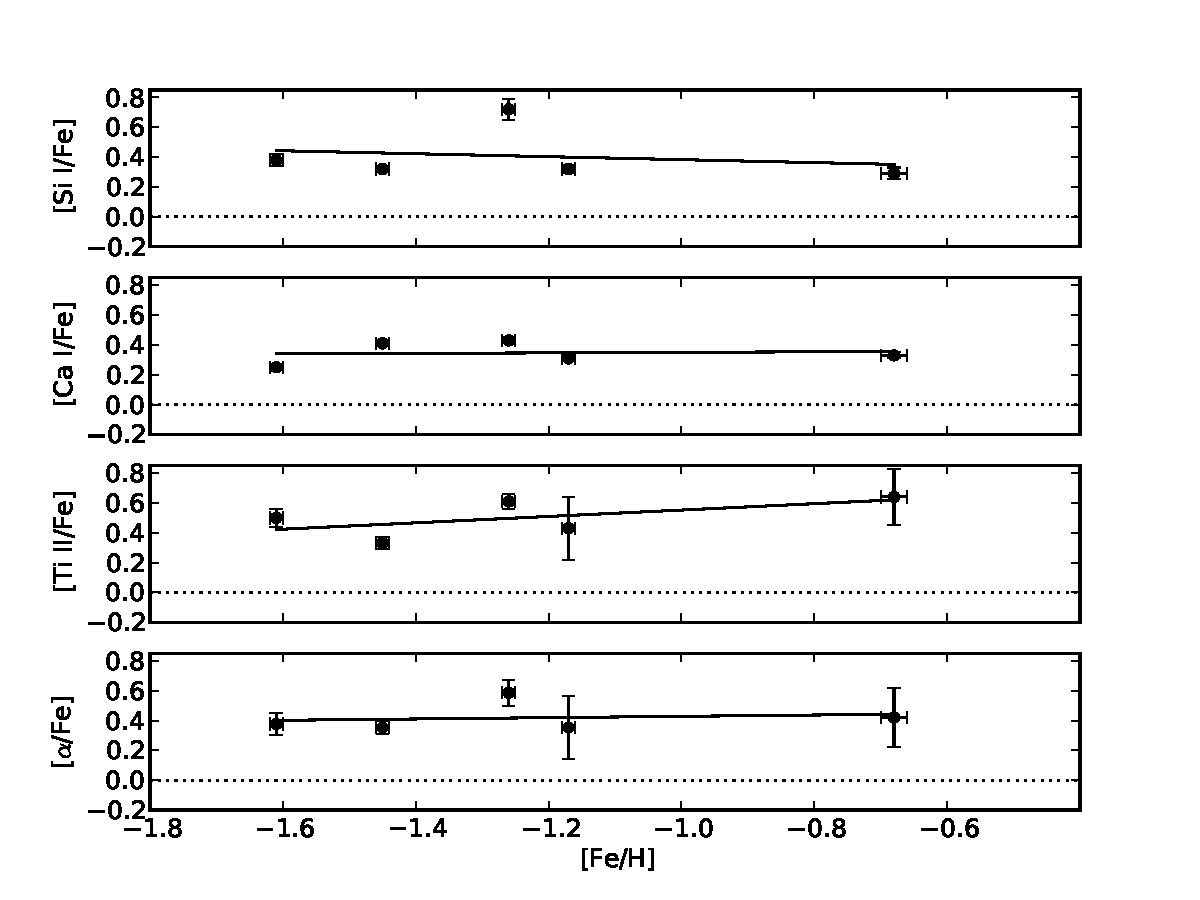
\includegraphics[width=\columnwidth]{./figures/aquarius-alpha-fe.pdf}
	\caption{A plot showing $[\alpha/\mbox{Fe}]$ for all Aquarius stream stars.}
	\label{fig:alpha-fe}
\end{figure}

% Mg-Al
\begin{figure}[h]
	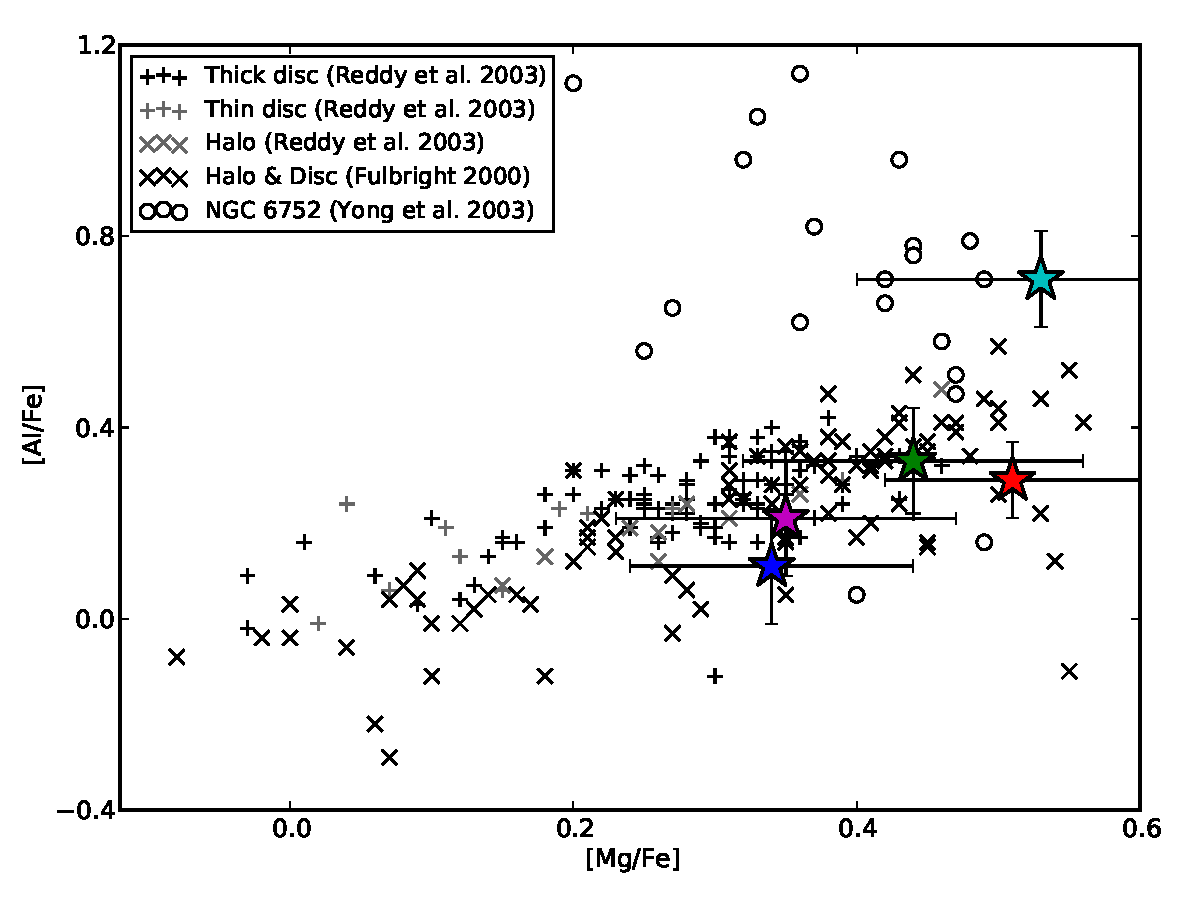
\includegraphics[width=\columnwidth]{./figures/aquarius-mg-al.pdf}
	\caption{A plot showing [Mg/Al] for all Aquarius stream stars.}
	\label{fig:mg-al}
\end{figure}

% [Na/Fe], [Cr/Fe], [Ni/Fe]
\begin{figure}[h]
	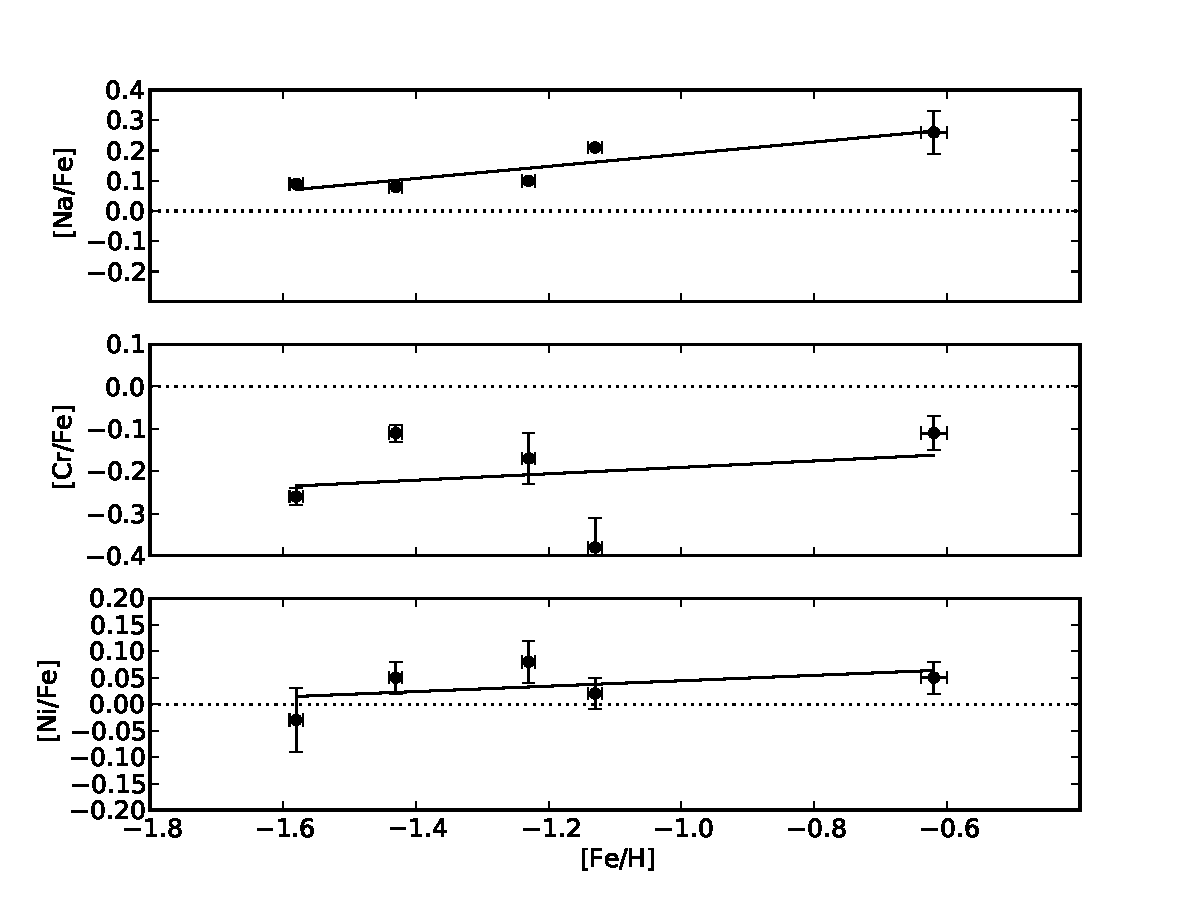
\includegraphics[width=\columnwidth]{./figures/aquarius-na-cr-ni-fe.pdf}
	\caption{A plot showing [Na/Fe], [Cr/Fe], and [Ni/Fe] for all Aquarius stream stars.}
	\label{fig:na-cr-ni-fe}
\end{figure}

% [Na/Fe], [Ni/Fe]
\begin{figure}[h]
	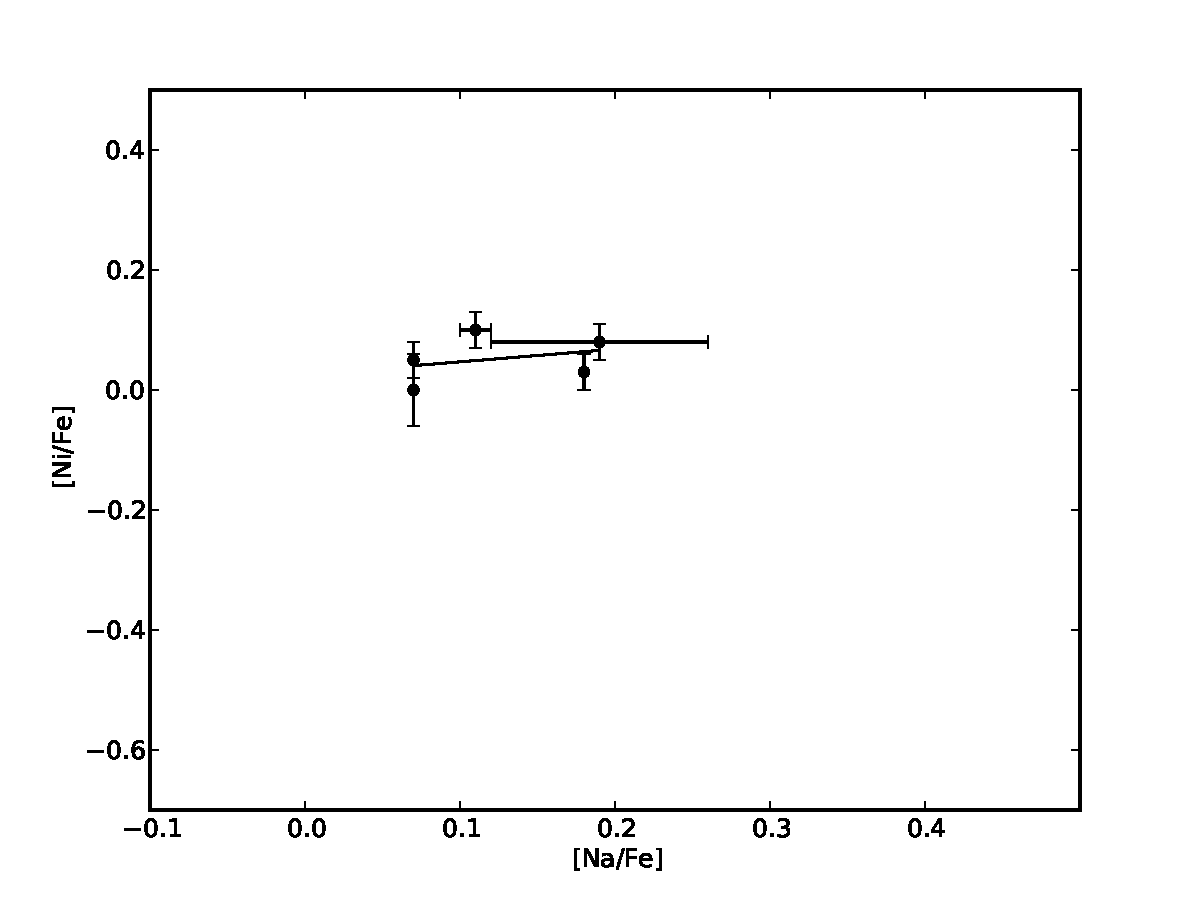
\includegraphics[width=\columnwidth]{./figures/aquarius-na-ni.pdf}
	\caption{A plot showing [Na/Fe] and [Ni/Fe] for all Aquarius stream stars.}
	\label{fig:na-ni}
\end{figure}

% [O/Fe], [Na/Fe]
\begin{figure}[h]
	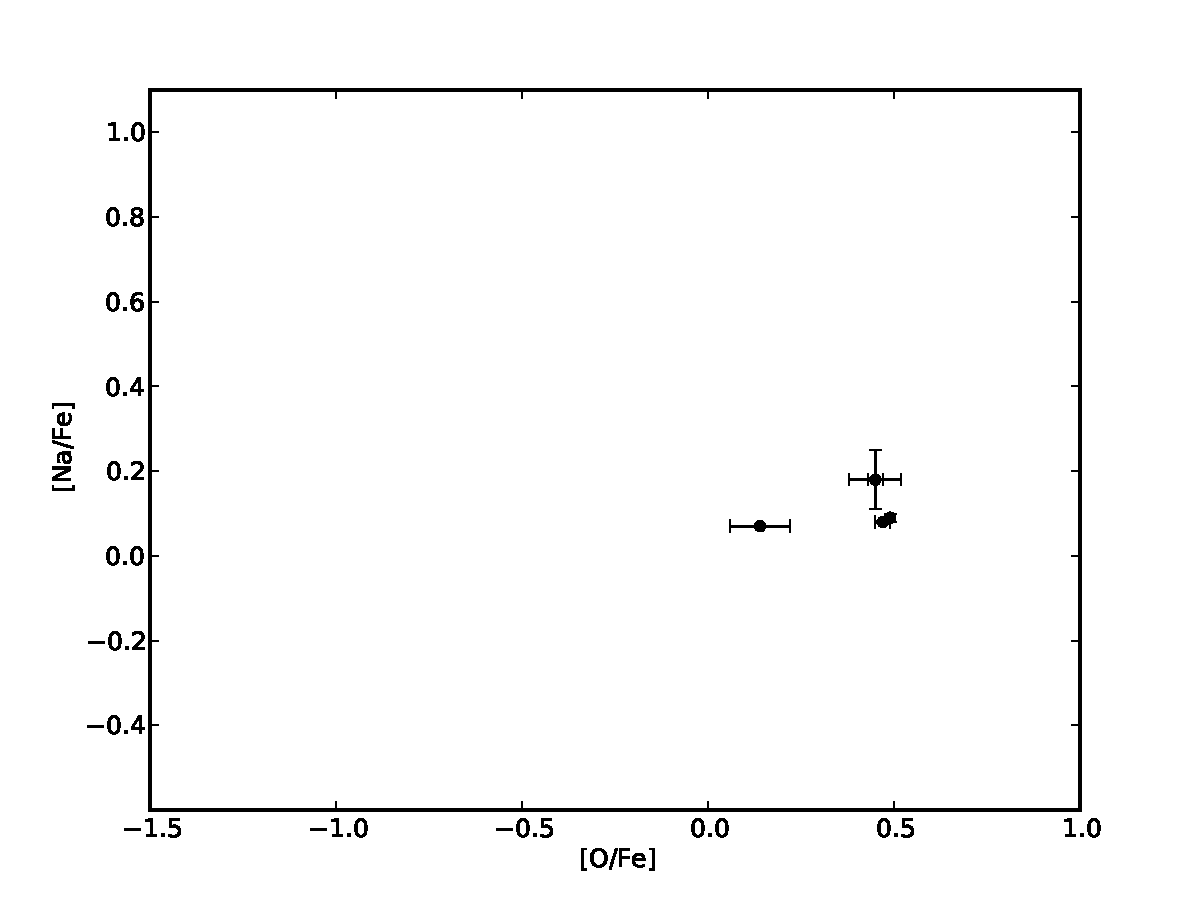
\includegraphics[width=\columnwidth]{./figures/aquarius-o-na.pdf}
	\caption{A plot showing [O/Fe] and [Na/Fe] for all Aquarius stream stars.}
	\label{fig:o-na}
\end{figure}

% Toombre
\begin{figure}[h]
	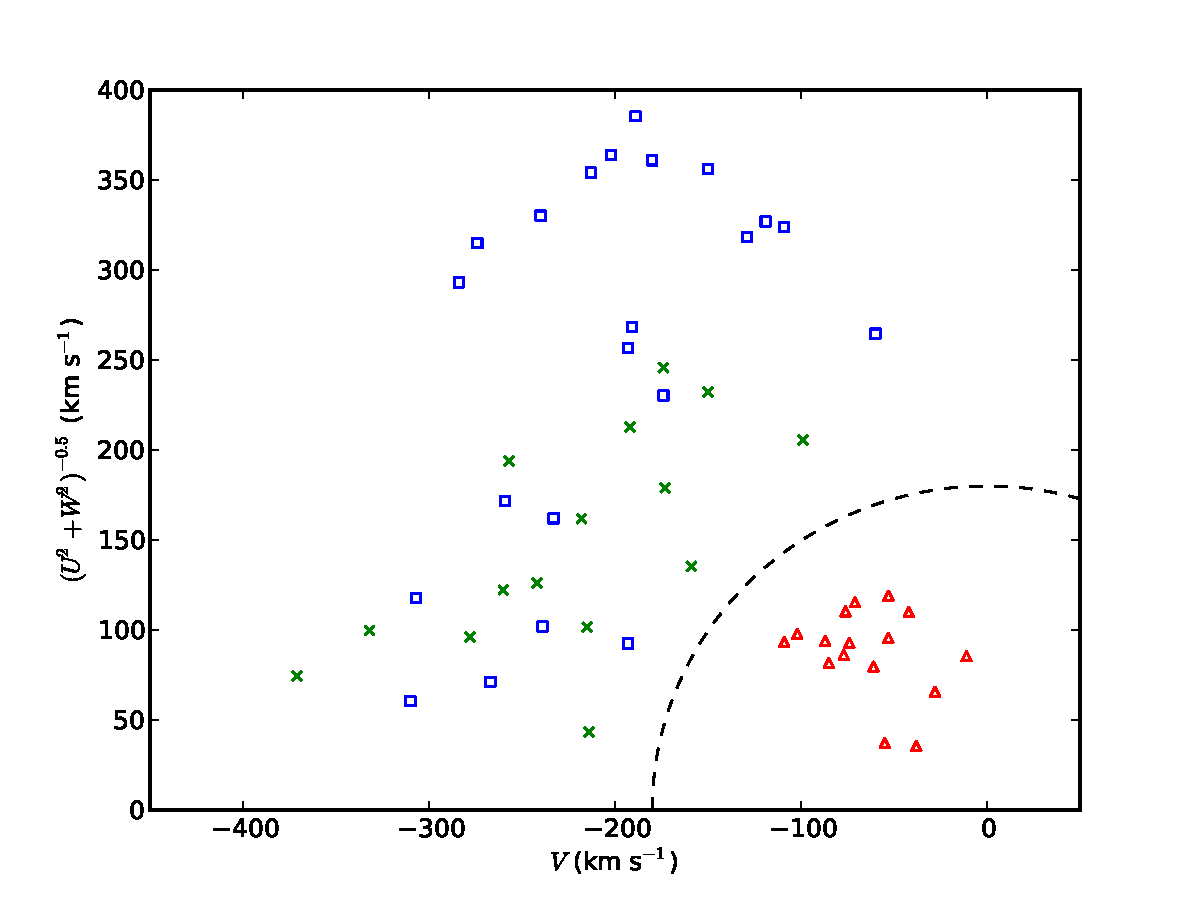
\includegraphics[width=\columnwidth]{./figures/plot-toombre.pdf}
	\caption{Toombre plot.}
	\label{fig:toombre}
\end{figure}


%\facilities{Magellan:Clay}

\bibliographystyle{apj}
\bibliography{bibliography}

\end{document}
